\documentclass{article}\usepackage[]{graphicx}\usepackage[]{color}
%% maxwidth is the original width if it is less than linewidth
%% otherwise use linewidth (to make sure the graphics do not exceed the margin)
\makeatletter
\def\maxwidth{ %
  \ifdim\Gin@nat@width>\linewidth
    \linewidth
  \else
    \Gin@nat@width
  \fi
}
\makeatother

\definecolor{fgcolor}{rgb}{0.345, 0.345, 0.345}
\newcommand{\hlnum}[1]{\textcolor[rgb]{0.686,0.059,0.569}{#1}}%
\newcommand{\hlstr}[1]{\textcolor[rgb]{0.192,0.494,0.8}{#1}}%
\newcommand{\hlcom}[1]{\textcolor[rgb]{0.678,0.584,0.686}{\textit{#1}}}%
\newcommand{\hlopt}[1]{\textcolor[rgb]{0,0,0}{#1}}%
\newcommand{\hlstd}[1]{\textcolor[rgb]{0.345,0.345,0.345}{#1}}%
\newcommand{\hlkwa}[1]{\textcolor[rgb]{0.161,0.373,0.58}{\textbf{#1}}}%
\newcommand{\hlkwb}[1]{\textcolor[rgb]{0.69,0.353,0.396}{#1}}%
\newcommand{\hlkwc}[1]{\textcolor[rgb]{0.333,0.667,0.333}{#1}}%
\newcommand{\hlkwd}[1]{\textcolor[rgb]{0.737,0.353,0.396}{\textbf{#1}}}%

\usepackage{framed}
\makeatletter
\newenvironment{kframe}{%
 \def\at@end@of@kframe{}%
 \ifinner\ifhmode%
  \def\at@end@of@kframe{\end{minipage}}%
  \begin{minipage}{\columnwidth}%
 \fi\fi%
 \def\FrameCommand##1{\hskip\@totalleftmargin \hskip-\fboxsep
 \colorbox{shadecolor}{##1}\hskip-\fboxsep
     % There is no \\@totalrightmargin, so:
     \hskip-\linewidth \hskip-\@totalleftmargin \hskip\columnwidth}%
 \MakeFramed {\advance\hsize-\width
   \@totalleftmargin\z@ \linewidth\hsize
   \@setminipage}}%
 {\par\unskip\endMakeFramed%
 \at@end@of@kframe}
\makeatother

\definecolor{shadecolor}{rgb}{.97, .97, .97}
\definecolor{messagecolor}{rgb}{0, 0, 0}
\definecolor{warningcolor}{rgb}{1, 0, 1}
\definecolor{errorcolor}{rgb}{1, 0, 0}
\newenvironment{knitrout}{}{} % an empty environment to be redefined in TeX

\usepackage{alltt}
\usepackage[vmargin=1in,hmargin=1in]{geometry}
\usepackage{enumerate}
\IfFileExists{upquote.sty}{\usepackage{upquote}}{}
\begin{document}
\title{Homework 5}
\date{BSAD 8700 - Business Analytics\\ Due: February 16, 2015}
\author{Kris Hanus, Laura Glathar, Arkya Rakshit, Jace Crist, Brandon Dlugosz\\ University of Nebraska at Omaha}
\maketitle

\textbf{ANSWER FOR 8:} \\

\begin{enumerate}[(a)]
\item
\begin{knitrout}
\definecolor{shadecolor}{rgb}{0.969, 0.969, 0.969}\color{fgcolor}\begin{kframe}
\begin{alltt}
\hlkwd{library}\hlstd{(MASS)}
\hlkwd{library}\hlstd{(dplyr)}
\end{alltt}


{\ttfamily\noindent\itshape\color{messagecolor}{\#\# \\\#\# Attaching package: 'dplyr'\\\#\# \\\#\# The following object is masked from 'package:MASS':\\\#\# \\\#\#\ \ \ \  select\\\#\# \\\#\# The following object is masked from 'package:stats':\\\#\# \\\#\#\ \ \ \  filter\\\#\# \\\#\# The following objects are masked from 'package:base':\\\#\# \\\#\#\ \ \ \  intersect, setdiff, setequal, union}}\begin{alltt}
\hlkwd{library}\hlstd{(ISLR)}
\hlkwd{library}\hlstd{(caret)}
\end{alltt}


{\ttfamily\noindent\itshape\color{messagecolor}{\#\# Loading required package: lattice\\\#\# Loading required package: ggplot2}}\begin{alltt}
\hlkwd{library}\hlstd{(tree)}
\end{alltt}
\end{kframe}
\end{knitrout}
For some odd reason echo $=$ FALSE is failing.
\begin{knitrout}
\definecolor{shadecolor}{rgb}{0.969, 0.969, 0.969}\color{fgcolor}\begin{kframe}
\begin{alltt}
\hlkwd{attach}\hlstd{(Carseats)}
\hlstd{High} \hlkwb{=} \hlkwd{ifelse} \hlstd{(Sales} \hlopt{<=} \hlnum{8}\hlstd{,}\hlstr{"No"}\hlstd{,} \hlstr{"Yes"}\hlstd{)}
\hlstd{Carseats} \hlkwb{=} \hlkwd{data.frame}\hlstd{(Carseats, High)}
\hlkwd{head}\hlstd{(Carseats)}
\end{alltt}
\begin{verbatim}
##   Sales CompPrice Income Advertising Population Price ShelveLoc Age
## 1  9.50       138     73          11        276   120       Bad  42
## 2 11.22       111     48          16        260    83      Good  65
## 3 10.06       113     35          10        269    80    Medium  59
## 4  7.40       117    100           4        466    97    Medium  55
## 5  4.15       141     64           3        340   128       Bad  38
## 6 10.81       124    113          13        501    72       Bad  78
##   Education Urban  US High
## 1        17   Yes Yes  Yes
## 2        10   Yes Yes  Yes
## 3        12   Yes Yes  Yes
## 4        14   Yes Yes   No
## 5        13   Yes  No   No
## 6        16    No Yes  Yes
\end{verbatim}
\begin{alltt}
\hlkwd{set.seed}\hlstd{(}\hlnum{2345}\hlstd{)}
\hlstd{DataIndex}\hlkwb{<-}\hlkwd{createDataPartition}\hlstd{(Carseats}\hlopt{$}\hlstd{Sales,} \hlkwc{p} \hlstd{=} \hlnum{0.8}\hlstd{,} \hlkwc{list}\hlstd{=}\hlnum{FALSE}\hlstd{,} \hlkwc{times}\hlstd{=}\hlnum{1}\hlstd{)}
\hlstd{train}\hlkwb{<-}\hlstd{Carseats[DataIndex,]}
\hlstd{Carseats.test}\hlkwb{<-}\hlstd{Carseats[}\hlopt{-}\hlstd{DataIndex,]}
\hlstd{High.test}\hlkwb{=}\hlstd{High[}\hlopt{-}\hlstd{DataIndex]}
\hlkwd{dim}\hlstd{(Carseats)}
\end{alltt}
\begin{verbatim}
## [1] 400  12
\end{verbatim}
\begin{alltt}
\hlkwd{dim}\hlstd{(train)}
\end{alltt}
\begin{verbatim}
## [1] 321  12
\end{verbatim}
\begin{alltt}
\hlkwd{dim}\hlstd{(Carseats.test)}
\end{alltt}
\begin{verbatim}
## [1] 79 12
\end{verbatim}
\end{kframe}
\end{knitrout}
Carseatstraining is a randomly chosen training data set, and Carseatstest is a randomly chosen test data set. Both were selected by non-replacement methods. This is a better method of selection (then what the book shows) creating no bias and no sequencing issues in the data.

\item
\begin{knitrout}
\definecolor{shadecolor}{rgb}{0.969, 0.969, 0.969}\color{fgcolor}\begin{kframe}
\begin{alltt}
\hlkwd{str}\hlstd{(Carseats)}
\end{alltt}
\begin{verbatim}
## 'data.frame':	400 obs. of  12 variables:
##  $ Sales      : num  9.5 11.22 10.06 7.4 4.15 ...
##  $ CompPrice  : num  138 111 113 117 141 124 115 136 132 132 ...
##  $ Income     : num  73 48 35 100 64 113 105 81 110 113 ...
##  $ Advertising: num  11 16 10 4 3 13 0 15 0 0 ...
##  $ Population : num  276 260 269 466 340 501 45 425 108 131 ...
##  $ Price      : num  120 83 80 97 128 72 108 120 124 124 ...
##  $ ShelveLoc  : Factor w/ 3 levels "Bad","Good","Medium": 1 2 3 3 1 1 3 2 3 3 ...
##  $ Age        : num  42 65 59 55 38 78 71 67 76 76 ...
##  $ Education  : num  17 10 12 14 13 16 15 10 10 17 ...
##  $ Urban      : Factor w/ 2 levels "No","Yes": 2 2 2 2 2 1 2 2 1 1 ...
##  $ US         : Factor w/ 2 levels "No","Yes": 2 2 2 2 1 2 1 2 1 2 ...
##  $ High       : Factor w/ 2 levels "No","Yes": 2 2 2 1 1 2 1 2 1 1 ...
\end{verbatim}
\begin{alltt}
\hlstd{tree.carseats}\hlkwb{=}\hlkwd{tree}\hlstd{(High}\hlopt{~}\hlstd{.}\hlopt{-}\hlstd{Sales, Carseats)}
\hlkwd{summary}\hlstd{(tree.carseats)}
\end{alltt}
\begin{verbatim}
## 
## Classification tree:
## tree(formula = High ~ . - Sales, data = Carseats)
## Variables actually used in tree construction:
## [1] "ShelveLoc"   "Price"       "Income"      "CompPrice"   "Population" 
## [6] "Advertising" "Age"         "US"         
## Number of terminal nodes:  27 
## Residual mean deviance:  0.4575 = 170.7 / 373 
## Misclassification error rate: 0.09 = 36 / 400
\end{verbatim}
\begin{alltt}
\hlkwd{plot}\hlstd{(tree.carseats)}
\hlkwd{text}\hlstd{(tree.carseats,} \hlkwc{pretty} \hlstd{=} \hlnum{0}\hlstd{,}\hlkwc{cex}\hlstd{=}\hlnum{0.6}\hlstd{,}\hlkwc{srt}\hlstd{=}\hlnum{75}\hlstd{)}
\end{alltt}
\end{kframe}
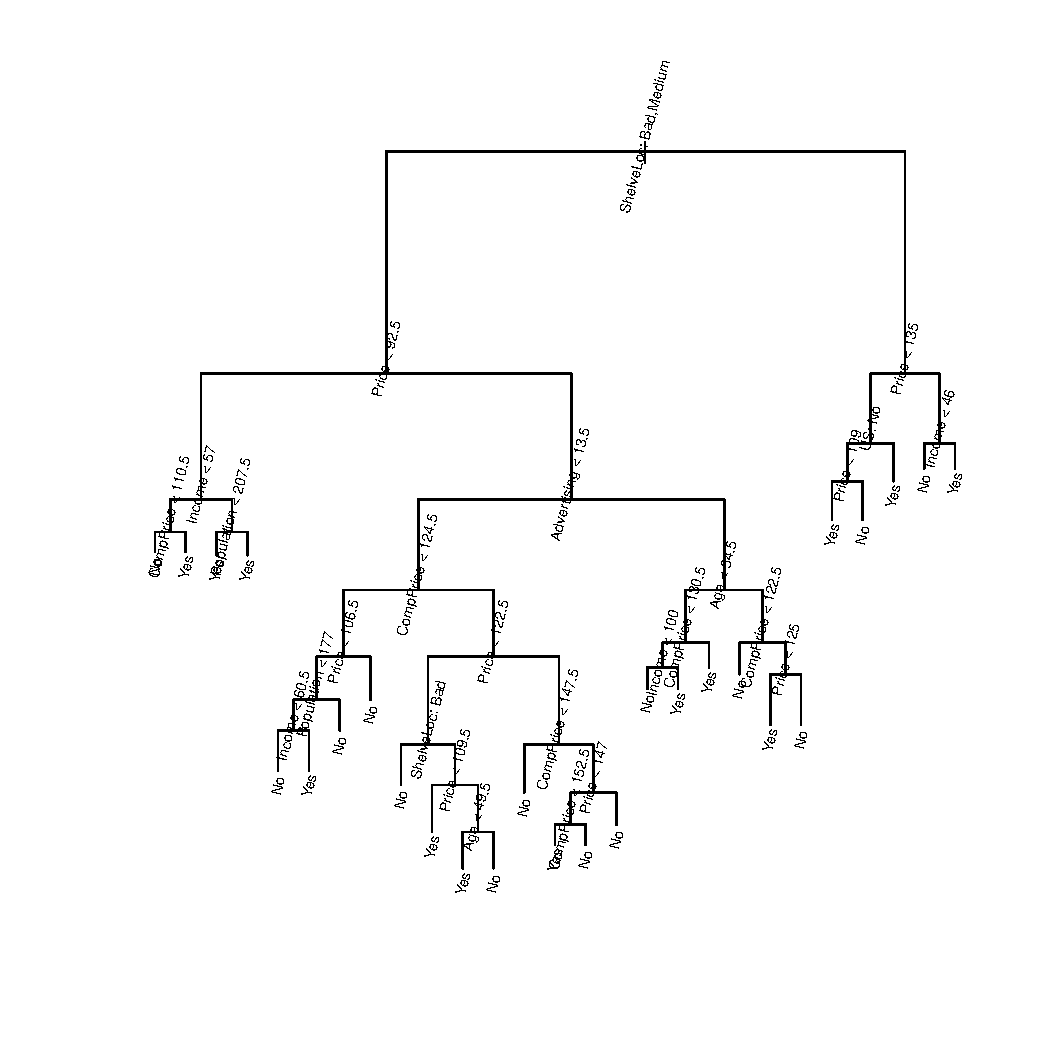
\includegraphics[width=\maxwidth]{figure/unnamed-chunk-3-1} 

\end{knitrout}
$MSE = 9\%$. By forcing the model to create an optimal dataset and model selection this should eliminating error.

\item
\begin{knitrout}
\definecolor{shadecolor}{rgb}{0.969, 0.969, 0.969}\color{fgcolor}\begin{kframe}
\begin{alltt}
\hlstd{tree.carseats}
\end{alltt}
\begin{verbatim}
## node), split, n, deviance, yval, (yprob)
##       * denotes terminal node
## 
##   1) root 400 541.500 No ( 0.59000 0.41000 )  
##     2) ShelveLoc: Bad,Medium 315 390.600 No ( 0.68889 0.31111 )  
##       4) Price < 92.5 46  56.530 Yes ( 0.30435 0.69565 )  
##         8) Income < 57 10  12.220 No ( 0.70000 0.30000 )  
##          16) CompPrice < 110.5 5   0.000 No ( 1.00000 0.00000 ) *
##          17) CompPrice > 110.5 5   6.730 Yes ( 0.40000 0.60000 ) *
##         9) Income > 57 36  35.470 Yes ( 0.19444 0.80556 )  
##          18) Population < 207.5 16  21.170 Yes ( 0.37500 0.62500 ) *
##          19) Population > 207.5 20   7.941 Yes ( 0.05000 0.95000 ) *
##       5) Price > 92.5 269 299.800 No ( 0.75465 0.24535 )  
##        10) Advertising < 13.5 224 213.200 No ( 0.81696 0.18304 )  
##          20) CompPrice < 124.5 96  44.890 No ( 0.93750 0.06250 )  
##            40) Price < 106.5 38  33.150 No ( 0.84211 0.15789 )  
##              80) Population < 177 12  16.300 No ( 0.58333 0.41667 )  
##               160) Income < 60.5 6   0.000 No ( 1.00000 0.00000 ) *
##               161) Income > 60.5 6   5.407 Yes ( 0.16667 0.83333 ) *
##              81) Population > 177 26   8.477 No ( 0.96154 0.03846 ) *
##            41) Price > 106.5 58   0.000 No ( 1.00000 0.00000 ) *
##          21) CompPrice > 124.5 128 150.200 No ( 0.72656 0.27344 )  
##            42) Price < 122.5 51  70.680 Yes ( 0.49020 0.50980 )  
##              84) ShelveLoc: Bad 11   6.702 No ( 0.90909 0.09091 ) *
##              85) ShelveLoc: Medium 40  52.930 Yes ( 0.37500 0.62500 )  
##               170) Price < 109.5 16   7.481 Yes ( 0.06250 0.93750 ) *
##               171) Price > 109.5 24  32.600 No ( 0.58333 0.41667 )  
##                 342) Age < 49.5 13  16.050 Yes ( 0.30769 0.69231 ) *
##                 343) Age > 49.5 11   6.702 No ( 0.90909 0.09091 ) *
##            43) Price > 122.5 77  55.540 No ( 0.88312 0.11688 )  
##              86) CompPrice < 147.5 58  17.400 No ( 0.96552 0.03448 ) *
##              87) CompPrice > 147.5 19  25.010 No ( 0.63158 0.36842 )  
##               174) Price < 147 12  16.300 Yes ( 0.41667 0.58333 )  
##                 348) CompPrice < 152.5 7   5.742 Yes ( 0.14286 0.85714 ) *
##                 349) CompPrice > 152.5 5   5.004 No ( 0.80000 0.20000 ) *
##               175) Price > 147 7   0.000 No ( 1.00000 0.00000 ) *
##        11) Advertising > 13.5 45  61.830 Yes ( 0.44444 0.55556 )  
##          22) Age < 54.5 25  25.020 Yes ( 0.20000 0.80000 )  
##            44) CompPrice < 130.5 14  18.250 Yes ( 0.35714 0.64286 )  
##              88) Income < 100 9  12.370 No ( 0.55556 0.44444 ) *
##              89) Income > 100 5   0.000 Yes ( 0.00000 1.00000 ) *
##            45) CompPrice > 130.5 11   0.000 Yes ( 0.00000 1.00000 ) *
##          23) Age > 54.5 20  22.490 No ( 0.75000 0.25000 )  
##            46) CompPrice < 122.5 10   0.000 No ( 1.00000 0.00000 ) *
##            47) CompPrice > 122.5 10  13.860 No ( 0.50000 0.50000 )  
##              94) Price < 125 5   0.000 Yes ( 0.00000 1.00000 ) *
##              95) Price > 125 5   0.000 No ( 1.00000 0.00000 ) *
##     3) ShelveLoc: Good 85  90.330 Yes ( 0.22353 0.77647 )  
##       6) Price < 135 68  49.260 Yes ( 0.11765 0.88235 )  
##        12) US: No 17  22.070 Yes ( 0.35294 0.64706 )  
##          24) Price < 109 8   0.000 Yes ( 0.00000 1.00000 ) *
##          25) Price > 109 9  11.460 No ( 0.66667 0.33333 ) *
##        13) US: Yes 51  16.880 Yes ( 0.03922 0.96078 ) *
##       7) Price > 135 17  22.070 No ( 0.64706 0.35294 )  
##        14) Income < 46 6   0.000 No ( 1.00000 0.00000 ) *
##        15) Income > 46 11  15.160 Yes ( 0.45455 0.54545 ) *
\end{verbatim}
\begin{alltt}
\hlkwd{set.seed} \hlstd{(}\hlnum{2}\hlstd{)}
\hlstd{tree.carseats} \hlkwb{=}\hlkwd{tree}\hlstd{(High}\hlopt{~}\hlstd{.}\hlopt{-}\hlstd{Sales, train)}
\hlstd{tree.pred}\hlkwb{=}\hlkwd{predict}\hlstd{(tree.carseats, Carseats.test,} \hlkwc{type} \hlstd{=} \hlstr{'class'} \hlstd{)}
\hlkwd{table}\hlstd{(tree.pred, High.test)}
\end{alltt}
\begin{verbatim}
##          High.test
## tree.pred No Yes
##       No  37   8
##       Yes 12  22
\end{verbatim}
\begin{alltt}
\hlstd{(}\hlnum{59}\hlstd{)}\hlopt{/}\hlnum{79}
\end{alltt}
\begin{verbatim}
## [1] 0.7468354
\end{verbatim}
\begin{alltt}
\hlkwd{set.seed} \hlstd{(}\hlnum{3}\hlstd{)}
\hlstd{cv.carseats} \hlkwb{=}\hlkwd{cv.tree}\hlstd{(tree.carseats ,}\hlkwc{FUN}\hlstd{=prune.misclass )}
\hlkwd{names}\hlstd{(cv.carseats )}
\end{alltt}
\begin{verbatim}
## [1] "size"   "dev"    "k"      "method"
\end{verbatim}
\begin{alltt}
\hlstd{cv.carseats}
\end{alltt}
\begin{verbatim}
## $size
##  [1] 26 23 20 18 12  8  6  3  2  1
## 
## $dev
##  [1]  87  87  82  85  88  89  88  91  98 134
## 
## $k
##  [1]      -Inf  0.000000  1.000000  1.500000  1.833333  2.000000  2.500000
##  [8]  5.333333 16.000000 40.000000
## 
## $method
## [1] "misclass"
## 
## attr(,"class")
## [1] "prune"         "tree.sequence"
\end{verbatim}
\begin{alltt}
\hlkwd{par}\hlstd{(}\hlkwc{mfrow} \hlstd{=}\hlkwd{c}\hlstd{(}\hlnum{1}\hlstd{,}\hlnum{2}\hlstd{))}
\hlkwd{plot}\hlstd{(cv.carseats}\hlopt{$}\hlstd{size ,cv.carseats}\hlopt{$}\hlstd{dev ,}\hlkwc{type}\hlstd{=}\hlstr{"b"}\hlstd{)}
\hlkwd{plot}\hlstd{(cv.carseats}\hlopt{$}\hlstd{k ,cv.carseats}\hlopt{$}\hlstd{dev ,}\hlkwc{type}\hlstd{=}\hlstr{"b"}\hlstd{)}
\end{alltt}
\end{kframe}
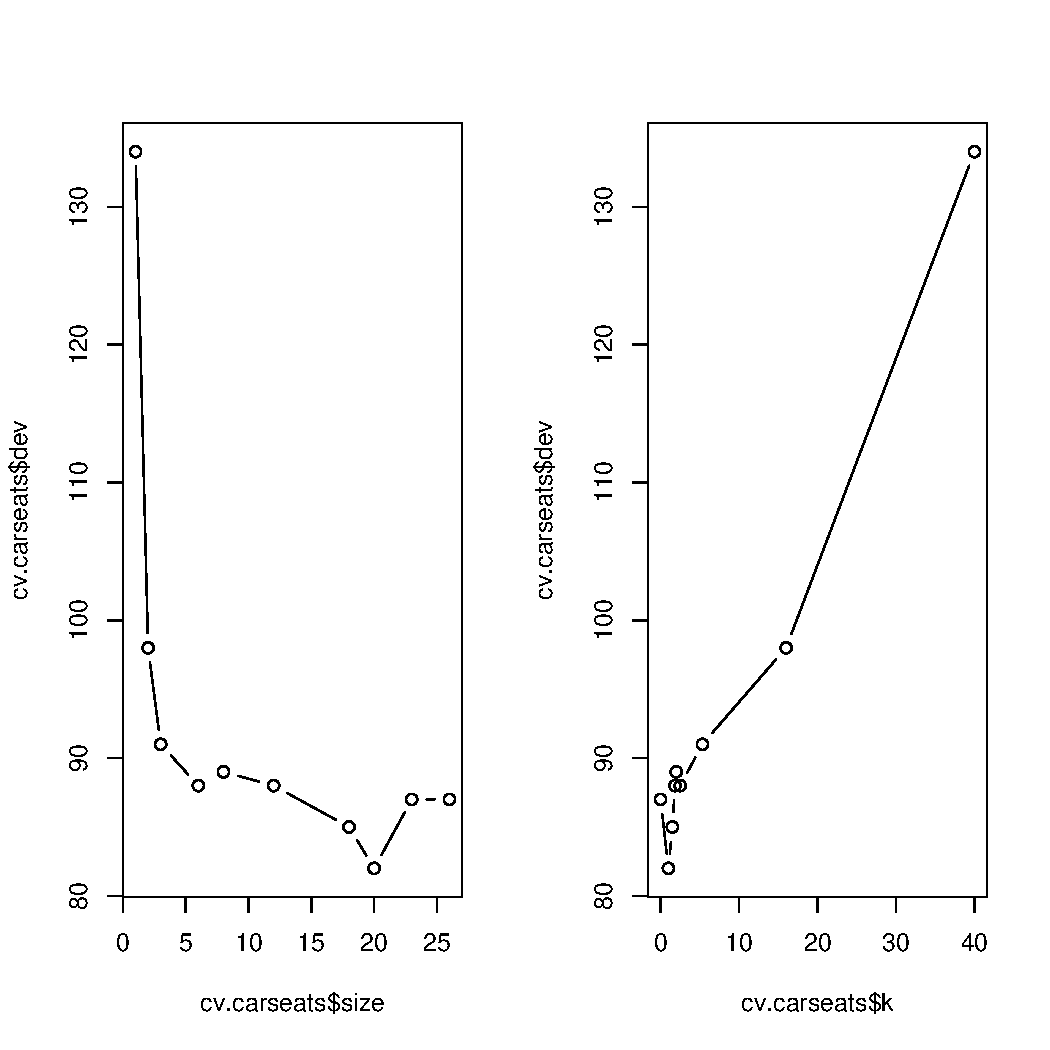
\includegraphics[width=\maxwidth]{figure/unnamed-chunk-4-1} 
\begin{kframe}\begin{alltt}
\hlstd{prune.carseats} \hlkwb{=}\hlkwd{prune.misclass} \hlstd{(tree.carseats ,}\hlkwc{best} \hlstd{=}\hlnum{6}\hlstd{)}
\hlkwd{plot}\hlstd{(prune.carseats )}
\hlkwd{text}\hlstd{(prune.carseats ,}\hlkwc{pretty} \hlstd{=}\hlnum{0}\hlstd{,}\hlkwc{cex}\hlstd{=}\hlnum{0.6}\hlstd{,}\hlkwc{srt}\hlstd{=}\hlnum{75}\hlstd{)}

\hlstd{tree.pred}\hlkwb{=}\hlkwd{predict} \hlstd{(prune.carseats , Carseats.test ,}\hlkwc{type}\hlstd{=}\hlstr{"class"}\hlstd{)}
\hlkwd{table}\hlstd{(tree.pred ,High.test)}
\end{alltt}
\begin{verbatim}
##          High.test
## tree.pred No Yes
##       No  36  10
##       Yes 13  20
\end{verbatim}
\begin{alltt}
\hlstd{prune.carseats} \hlkwb{=}\hlkwd{prune.misclass} \hlstd{(tree.carseats ,}\hlkwc{best} \hlstd{=}\hlnum{20}\hlstd{)}
\hlkwd{plot}\hlstd{(prune.carseats )}
\hlkwd{text}\hlstd{(prune.carseats ,}\hlkwc{pretty} \hlstd{=}\hlnum{0}\hlstd{,}\hlkwc{cex}\hlstd{=}\hlnum{0.75}\hlstd{,}\hlkwc{srt}\hlstd{=}\hlnum{75}\hlstd{)}
\end{alltt}
\end{kframe}
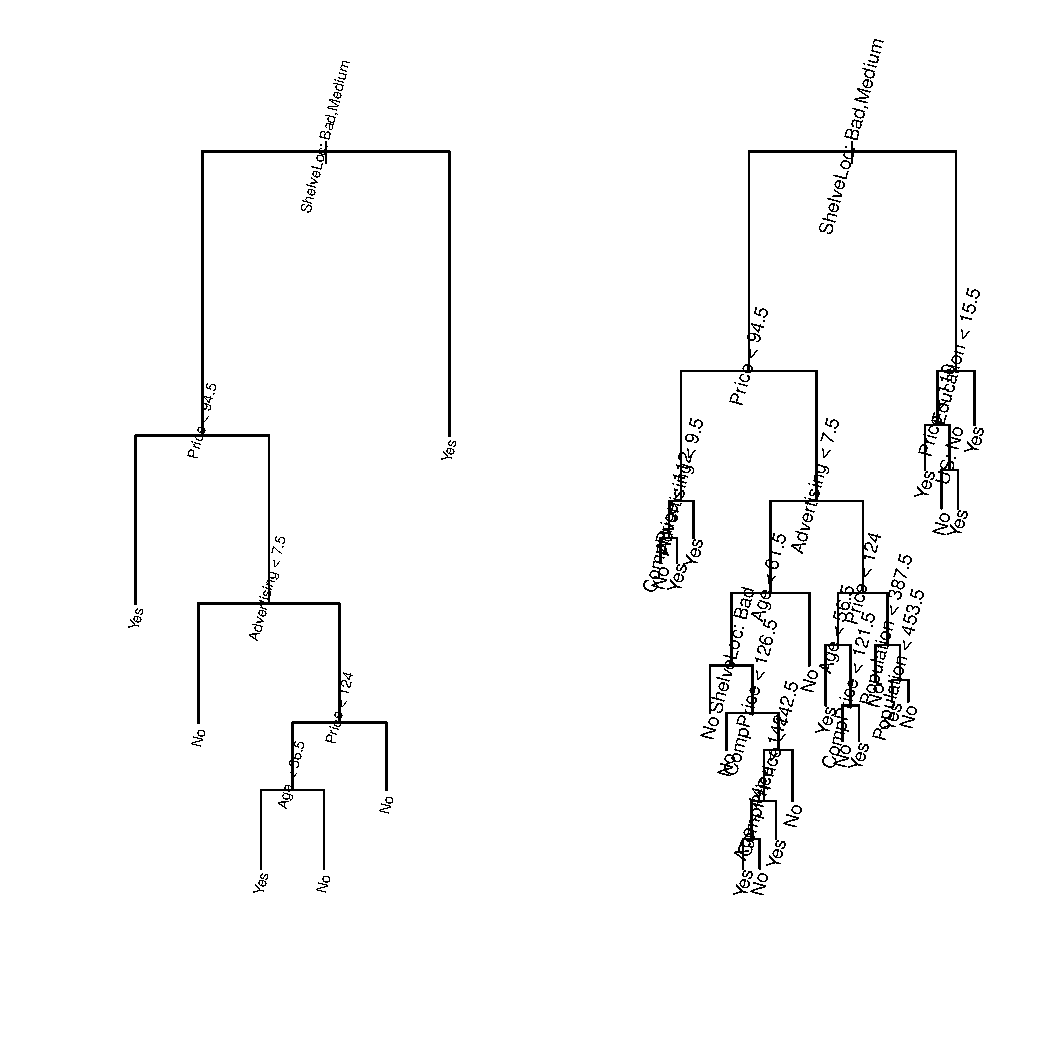
\includegraphics[width=\maxwidth]{figure/unnamed-chunk-4-2} 
\begin{kframe}\begin{alltt}
\hlstd{tree.pred}\hlkwb{=}\hlkwd{predict} \hlstd{(prune.carseats , Carseats.test ,}\hlkwc{type}\hlstd{=}\hlstr{"class"}\hlstd{)}
\hlkwd{table}\hlstd{(tree.pred ,High.test)}
\end{alltt}
\begin{verbatim}
##          High.test
## tree.pred No Yes
##       No  37  10
##       Yes 12  20
\end{verbatim}
\end{kframe}
\end{knitrout}
With pruning, my results from part b it seems that the fitted model to the training data is predicting with a $75\%$ accuracy. This is $3.5\%$ better then the books method. Pruning my model is only pushing around the error. It is not improving the model. However, using bagging methods instead might be the better method.
\end{enumerate}
\newpage
\textbf{ANSWER FOR 9:} \\

\begin{enumerate}[(a)]
\item
\begin{knitrout}
\definecolor{shadecolor}{rgb}{0.969, 0.969, 0.969}\color{fgcolor}\begin{kframe}
\begin{alltt}
\hlkwd{tail}\hlstd{(OJ,} \hlnum{3}\hlstd{)}
\end{alltt}
\begin{verbatim}
##      Purchase WeekofPurchase StoreID PriceCH PriceMM DiscCH DiscMM
## 1068       MM            257       7    1.86    2.18      0   0.00
## 1069       CH            261       7    1.86    2.13      0   0.24
## 1070       CH            270       1    1.86    2.18      0   0.00
##      SpecialCH SpecialMM  LoyalCH SalePriceMM SalePriceCH PriceDiff Store7
## 1068         0         0 0.736206        2.18        1.86      0.32    Yes
## 1069         0         0 0.588965        1.89        1.86      0.03    Yes
## 1070         0         0 0.671172        2.18        1.86      0.32     No
##      PctDiscMM PctDiscCH ListPriceDiff STORE
## 1068  0.000000         0          0.32     0
## 1069  0.112676         0          0.27     0
## 1070  0.000000         0          0.32     1
\end{verbatim}
\begin{alltt}
\hlnum{800}\hlopt{/}\hlnum{1070}
\end{alltt}
\begin{verbatim}
## [1] 0.7476636
\end{verbatim}
\begin{alltt}
\hlkwd{attach}\hlstd{(OJ)}
\hlkwd{set.seed}\hlstd{(}\hlnum{5432}\hlstd{)}
\hlstd{DataIndex2}\hlkwb{<-}\hlkwd{createDataPartition}\hlstd{(OJ}\hlopt{$}\hlstd{Purchase,} \hlkwc{p} \hlstd{=} \hlnum{0.747}\hlstd{,} \hlkwc{list}\hlstd{=}\hlnum{FALSE}\hlstd{,} \hlkwc{times}\hlstd{=}\hlnum{1}\hlstd{)}
\hlstd{train2}\hlkwb{<-}\hlstd{OJ[DataIndex2,]}
\hlstd{OJ.test}\hlkwb{<-}\hlstd{OJ[}\hlopt{-}\hlstd{DataIndex2,]}
\hlkwd{dim}\hlstd{(train2)}
\end{alltt}
\begin{verbatim}
## [1] 800  18
\end{verbatim}
\begin{alltt}
\hlkwd{dim}\hlstd{(OJ.test)}
\end{alltt}
\begin{verbatim}
## [1] 270  18
\end{verbatim}
\end{kframe}
\end{knitrout}
We decided to use a random sample because it will get rid of any bias or sequencing unknown to us in our sampling.

\item
\begin{knitrout}
\definecolor{shadecolor}{rgb}{0.969, 0.969, 0.969}\color{fgcolor}\begin{kframe}
\begin{alltt}
\hlstd{tree.OJ}\hlkwb{=}\hlkwd{tree}\hlstd{(Purchase}\hlopt{~}\hlstd{.,train2)}
\hlkwd{summary}\hlstd{(tree.OJ)}
\end{alltt}
\begin{verbatim}
## 
## Classification tree:
## tree(formula = Purchase ~ ., data = train2)
## Variables actually used in tree construction:
## [1] "LoyalCH"     "SalePriceMM" "SpecialCH"   "PriceDiff"  
## Number of terminal nodes:  8 
## Residual mean deviance:  0.7258 = 574.8 / 792 
## Misclassification error rate: 0.165 = 132 / 800
\end{verbatim}
\end{kframe}
\end{knitrout}
There were 8 terminal nodes with a $MSE = 16.25\%$.

\item
\begin{knitrout}
\definecolor{shadecolor}{rgb}{0.969, 0.969, 0.969}\color{fgcolor}\begin{kframe}
\begin{alltt}
\hlstd{tree.OJ}
\end{alltt}
\begin{verbatim}
## node), split, n, deviance, yval, (yprob)
##       * denotes terminal node
## 
##  1) root 800 1070.00 CH ( 0.61000 0.39000 )  
##    2) LoyalCH < 0.5036 353  415.10 MM ( 0.27479 0.72521 )  
##      4) LoyalCH < 0.275386 172  123.60 MM ( 0.11628 0.88372 )  
##        8) LoyalCH < 0.0490615 60   10.17 MM ( 0.01667 0.98333 ) *
##        9) LoyalCH > 0.0490615 112  102.00 MM ( 0.16964 0.83036 ) *
##      5) LoyalCH > 0.275386 181  246.90 MM ( 0.42541 0.57459 )  
##       10) SalePriceMM < 2.04 94  108.90 MM ( 0.26596 0.73404 )  
##         20) SpecialCH < 0.5 78   76.37 MM ( 0.19231 0.80769 ) *
##         21) SpecialCH > 0.5 16   21.17 CH ( 0.62500 0.37500 ) *
##       11) SalePriceMM > 2.04 87  117.30 CH ( 0.59770 0.40230 ) *
##    3) LoyalCH > 0.5036 447  337.30 CH ( 0.87472 0.12528 )  
##      6) LoyalCH < 0.764572 193  218.70 CH ( 0.74611 0.25389 )  
##       12) PriceDiff < 0.145 77  106.60 CH ( 0.51948 0.48052 ) *
##       13) PriceDiff > 0.145 116   77.16 CH ( 0.89655 0.10345 ) *
##      7) LoyalCH > 0.764572 254   64.09 CH ( 0.97244 0.02756 ) *
\end{verbatim}
\end{kframe}
\end{knitrout}
We picked terminal node begining after leaf 10. It seems that $76.37\%$ of customers will pick Minute Maid OJ unless there is a significant discount offered for Citrus Hill.

\item
\begin{knitrout}
\definecolor{shadecolor}{rgb}{0.969, 0.969, 0.969}\color{fgcolor}\begin{kframe}
\begin{alltt}
\hlkwd{plot}\hlstd{(tree.OJ)}
\hlkwd{text}\hlstd{(tree.OJ,}\hlkwc{pretty} \hlstd{=}\hlnum{0}\hlstd{,}\hlkwc{cex}\hlstd{=}\hlnum{0.6}\hlstd{,}\hlkwc{srt}\hlstd{=}\hlnum{75}\hlstd{)}
\end{alltt}
\end{kframe}
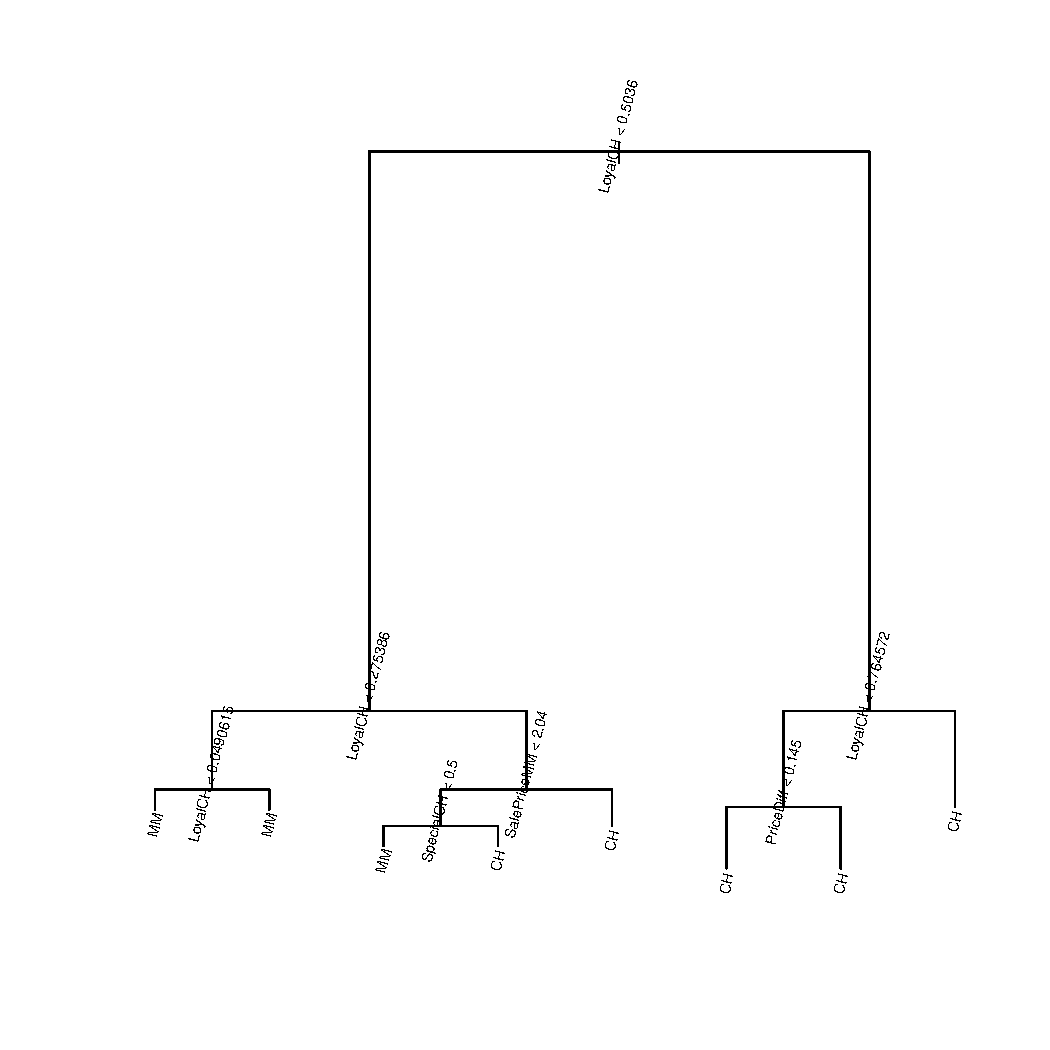
\includegraphics[width=\maxwidth]{figure/unnamed-chunk-8-1} 

\end{knitrout}
There seems to be a focus on the type of customer loyalty for CH based on deals and discounts. Also, in general customers will go will Minute Maid unless there is a savings.

\item
\begin{knitrout}
\definecolor{shadecolor}{rgb}{0.969, 0.969, 0.969}\color{fgcolor}\begin{kframe}
\begin{alltt}
\hlstd{tree.pred2}\hlkwb{=}\hlkwd{predict}\hlstd{(tree.OJ, OJ.test,} \hlkwc{type} \hlstd{=} \hlstr{'class'} \hlstd{)}
\hlkwd{table}\hlstd{(tree.pred2,OJ.test}\hlopt{$}\hlstd{Purchase)}
\end{alltt}
\begin{verbatim}
##           
## tree.pred2  CH  MM
##         CH 154  42
##         MM  11  63
\end{verbatim}
\begin{alltt}
\hlstd{(}\hlnum{154}\hlopt{+}\hlnum{63}\hlstd{)}\hlopt{/}\hlnum{270}
\end{alltt}
\begin{verbatim}
## [1] 0.8037037
\end{verbatim}
\end{kframe}
\end{knitrout}
We are able to predict with an $80.4\%$ accuracy. 

\item
\begin{knitrout}
\definecolor{shadecolor}{rgb}{0.969, 0.969, 0.969}\color{fgcolor}\begin{kframe}
\begin{alltt}
\hlkwd{set.seed} \hlstd{(}\hlnum{3}\hlstd{)}
\hlstd{cv.OJ} \hlkwb{=}\hlkwd{cv.tree}\hlstd{(tree.OJ ,}\hlkwc{FUN}\hlstd{=prune.misclass )}
\hlkwd{names}\hlstd{(cv.OJ)}
\end{alltt}
\begin{verbatim}
## [1] "size"   "dev"    "k"      "method"
\end{verbatim}
\begin{alltt}
\hlstd{cv.OJ}
\end{alltt}
\begin{verbatim}
## $size
## [1] 8 5 4 2 1
## 
## $dev
## [1] 154 154 161 163 312
## 
## $k
## [1]  -Inf   0.0   4.0   8.5 159.0
## 
## $method
## [1] "misclass"
## 
## attr(,"class")
## [1] "prune"         "tree.sequence"
\end{verbatim}
\end{kframe}
\end{knitrout}

The optimal tree size would have 4 terminal nodes. Dev is the lowest when size is 4.

\item
\begin{knitrout}
\definecolor{shadecolor}{rgb}{0.969, 0.969, 0.969}\color{fgcolor}\begin{kframe}
\begin{alltt}
\hlkwd{par}\hlstd{(}\hlkwc{mfrow} \hlstd{=}\hlkwd{c}\hlstd{(}\hlnum{1}\hlstd{,}\hlnum{2}\hlstd{))}
\hlkwd{plot}\hlstd{(cv.OJ}\hlopt{$}\hlstd{size ,cv.OJ}\hlopt{$}\hlstd{dev ,}\hlkwc{type}\hlstd{=}\hlstr{"b"}\hlstd{)}
\hlkwd{plot}\hlstd{(cv.OJ}\hlopt{$}\hlstd{k ,cv.OJ}\hlopt{$}\hlstd{dev ,}\hlkwc{type}\hlstd{=}\hlstr{"b"}\hlstd{)}
\end{alltt}
\end{kframe}
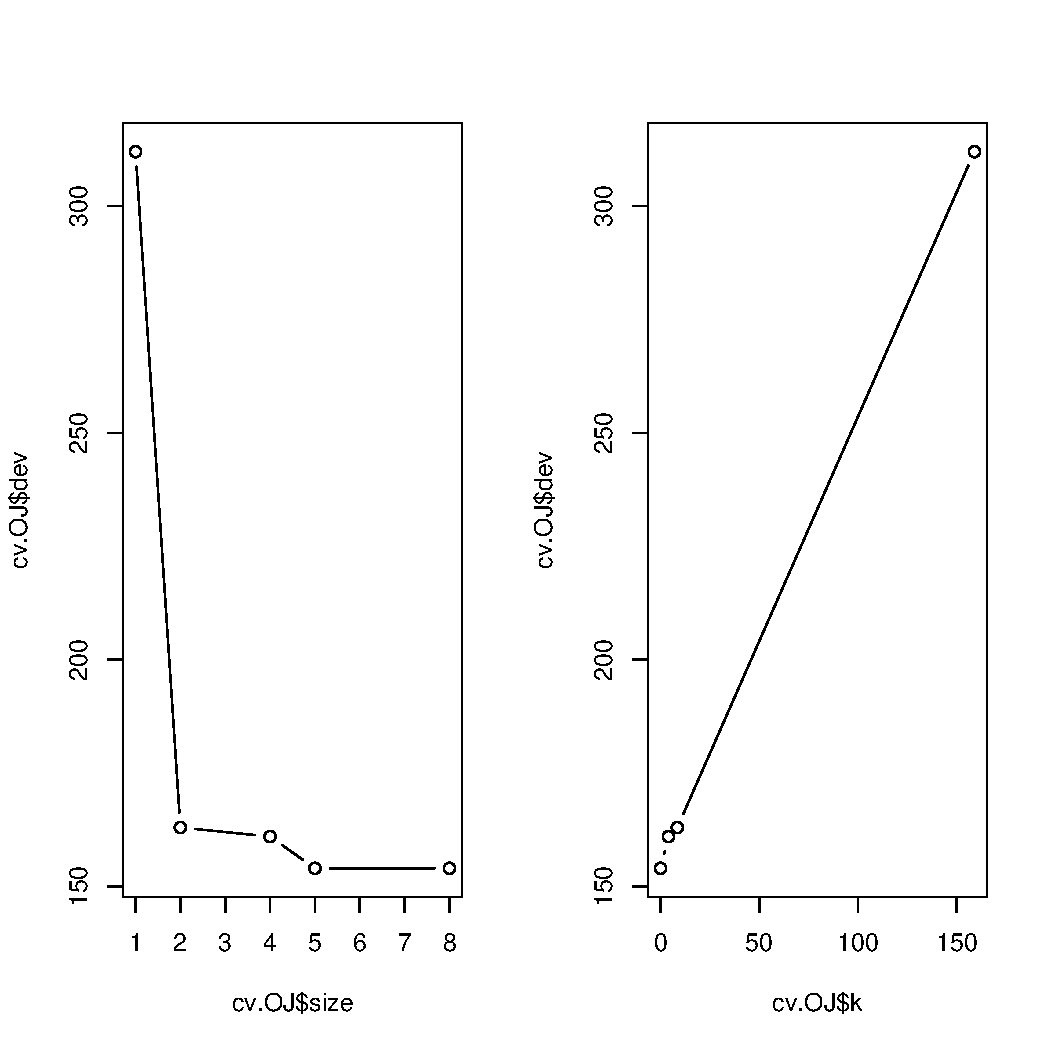
\includegraphics[width=\maxwidth]{figure/unnamed-chunk-11-1} 

\end{knitrout}
The first plot is a plot with tree size on the x-axis and cross-validated
classification error rate on the y-axis.

\item
As stated in part f, the optimal tree size would have 4 terminal nodes.

\end{enumerate}

\end{document}
